\documentclass[final,5p]{elsarticle}

% \documentclass[preprint,12pt]{elsarticle}

%% Use the option review to obtain double line spacing
%% \documentclass[authoryear,preprint,review,12pt]{elsarticle}

%% Use the options 1p,twocolumn; 3p; 3p,twocolumn; 5p; or 5p,twocolumn
%% for a journal layout:
% \documentclass[final,1p,times]{elsarticle}
%% \documentclass[final,1p,times,twocolumn]{elsarticle}
% \documentclass[final,3p,times]{elsarticle}
%% \documentclass[final,3p,times,twocolumn]{elsarticle}
% \documentclass[final,5p,times]{elsarticle}
%% \documentclass[final,5p,times,twocolumn]{elsarticle}
\usepackage[portuguese]{babel}

%% For including figures, graphicx.sty has been loaded in
%% elsarticle.cls. If you prefer to use the old commands
%% please give \usepackage{epsfig}

%% The amssymb package provides various useful mathematical symbols
\usepackage{amssymb}
\usepackage{amsmath}
\usepackage{multirow}
\usepackage{tabularx}
\usepackage{booktabs}
\usepackage{tablefootnote}

\usepackage{pgfplots}
\pgfplotsset{compat=1.18}
\usepgfplotslibrary{statistics}
\usepackage{pgfplotstable}

\usepackage{placeins}
\usepackage{hyperref}
\numberwithin{equation}{section}

\usepackage{algorithm}
\usepackage[noEnd=true, indLines=true]{algpseudocodex}
\algrenewcommand\algorithmicrequire{\textbf{Entrada:}}
\algrenewcommand\algorithmicwhile{\textbf{Enquanto}}
\algrenewcommand\algorithmicrepeat{\textbf{Repete}}
\algrenewcommand\algorithmicuntil{\textbf{Até}}
\algrenewcommand\algorithmicif{\textbf{Se}}
\algrenewcommand\algorithmicthen{\textbf{então}}
\algrenewcommand\algorithmicelse{\textbf{Caso contrário}}
\algrenewcommand\algorithmicensure{\textbf{Objetivo:}}
\algrenewcommand\algorithmicreturn{\textbf{Retorna:}}
\algrenewcommand\algorithmicdo{\textbf{faça}}
\algrenewcommand\algorithmicforall{\textbf{Para todos}}
\algnewcommand{\LineComment}[1]{\State \(\triangleright\) \textcolor{black!50}{\emph{#1}}}

\newcommand*{\squareb}{\textcolor{black}{\rule{0.5em}{0.5em}}}
\newcommand*{\squareg}{\textcolor{gray}{\rule{0.5em}{0.5em}}}

\graphicspath{ {./png/} }

% \usepackage[fleqn]{nccmath}
% \usepackage{multicol}


%=========== Gloabal Tikz settings
% \pgfplotsset{compat=newest}
% \usetikzlibrary{math}
% \pgfplotsset{
%     height = 10cm,
%     width = 10cm,
%     tick pos = left,
%     legend style={at={(0.98,0.30)}, anchor=east},
%     legend cell align=left,
%     }
%  \pgfkeys{
%     /pgf/number format/.cd,
%     fixed,
%     precision = 1,
%     set thousands separator = {}
% }

%% The amsthm package provides extended theorem environments
%% \usepackage{amsthm}

%% The lineno packages adds line numbers. Start line numbering with
%% \begin{linenumbers}, end it with \end{linenumbers}. Or switch it on
%% for the whole article with \linenumbers.
%% \usepackage{lineno}

\usepackage{listings}
\usepackage{xcolor}

\definecolor{codegreen}{rgb}{0,0.6,0}
\definecolor{codegray}{rgb}{0.5,0.5,0.5}
\definecolor{codepurple}{rgb}{0.58,0,0.82}
\definecolor{backcolour}{rgb}{0.98,0.98,0.98}

\lstdefinestyle{mystyle}{
    backgroundcolor=\color{backcolour},
    commentstyle=\color{codegreen},
    keywordstyle=\color{magenta},
    numberstyle=\tiny\color{codegray},
    stringstyle=\color{codepurple},
    basicstyle=\ttfamily\footnotesize,
    breakatwhitespace=false,
    breaklines=true,
    captionpos=b,
    keepspaces=true,
    numbers=left,
    numbersep=5pt,
    showspaces=false,
    showstringspaces=false,
    showtabs=false,
    tabsize=2
}

\lstset{style=mystyle}

% \journal{Nuclear Physics B}

\begin{document}

\begin{frontmatter}

%% Title, authors and addresses

%% use the tnoteref command within \title for footnotes;
%% use the tnotetext command for theassociated footnote;
%% use the fnref command within \author or \address for footnotes;
%% use the fntext command for theassociated footnote;
%% use the corref command within \author for corresponding author footnotes;
%% use the cortext command for theassociated footnote;
%% use the ead command for the email address,
%% and the form \ead[url] for the home page:
%% \title{Title\tnoteref{label1}}
%% \tnotetext[label1]{}
%% \author{Name\corref{cor1}\fnref{label2}}
%% \ead{email address}
%% \ead[url]{home page}
%% \fntext[label2]{}
%% \cortext[cor1]{}
%% \affiliation{organization={},
%%             addressline={},
%%             city={},
%%             postcode={},
%%             state={},
%%             country={}}
%% \fntext[label3]{}

\title{Avaliação de Técnicas de Classificação\tnoteref{label_title}}
\tnotetext[label_title]{Relatório número 02 como parte dos requisitos da disciplina IA048: Aprendizado de Máquina.}

%% use optional labels to link authors explicitly to addresses:
%% \author[label1,label2]{}
%% \affiliation[label1]{organization={},
%%             addressline={},
%%             city={},
%%             postcode={},
%%             state={},
%%             country={}}
%%
%% \affiliation[label2]{organization={},
%%             addressline={},
%%             city={},
%%             postcode={},
%%             state={},
%%             country={}}

\author[label1]{Tiago C A Amorim (RA: 100675)}
\affiliation[label1]{organization={Doutorando no Departamento de Engenharia de Petróleo da Faculdade de Engenharia Mecânica, UNICAMP},
            city={Campinas},
            state={SP},
            country={Brasil}}

\author[label2]{Taylon L C Martins (RA: 177379)}
\affiliation[label2]{organization={Aluno especial, UNICAMP},
            city={Campinas},
            state={SP},
            country={Brasil}}


% \begin{abstract}

%     xxxxxxx

% \end{abstract}


%%Graphical abstract
% \begin{graphicalabstract}
%\includegraphics{grabs}
% \end{graphicalabstract}

%%Research highlights
% \begin{highlights}
% \item Research highlight 1
% \item Research highlight 2
% \end{highlights}

\begin{keyword}
    Classificação \sep Regressão Logística \sep k-Vizinhos mais Próximos \sep Validação Cruzada
%% keywords here, in the form: keyword \sep keyword

%% PACS codes here, in the form: \PACS code \sep code

%% MSC codes here, in the form: \MSC code \sep code
%% or \MSC[2008] code \sep code (2000 is the default)

\end{keyword}

\end{frontmatter}

%% main text
\section{Introdução}

    Este relatório apresenta as principais atividades realizadas no desenvolvimento das atividades propostas na Lista 02 da disciplina IA048: Aprendizado de Máquina, primeiro semestre de 2024. O foco deste exercício é de construir a avaliar o desempenho de algoritmos de classificação usando duas versões de um mesmo estudo.

\section{Tarefa Proposta}

    Nesta atividade, vamos abordar o problema de reconhecimento de atividades humanas (HAR, do inglês \emph{human activity recognition}) a partir de informações capturadas por sensores de smartphones. Em particular, vamos trabalhar com a base de dados \href{https://archive.ics.uci.edu/dataset/240/human+activity+recognition+using+smartphones}{UCI HAR} \cite{anguita2013public}, que contém registros de sensores inerciais presentes em um smartphone preso à cintura de 30 sujeitos realizando atividades cotidianas. Cada pessoa realizou seis atividades, as quais correspondem aos seguintes rótulos:

    \begin{table}[h]
        \centering
        \begin{tabular}{l l c}
            \toprule
            \textbf{Atividade}\tablefootnote{Foram adicionados os termos originais entre parênteses para facilitar a comparação com os gráficos, que foram construídos com os termos em inglês.} & & \textbf{Rótulo} \\
            \midrule
            Caminhar & (\emph{Walking}) & 1 \\
            Subir escadas & (\emph{W. upstairs}) & 2 \\
            Descer escadas & (\emph{W. downstairs}) & 3 \\
            Sentado & (\emph{Sitting}) & 4 \\
            Em pé & (\emph{Standing}) & 5 \\
            Deitado & (\emph{Laying}) & 6 \\
            \bottomrule
        \end{tabular}
        \caption{Rótulos da base de dados.}
        \label{tab:rotulos}
    \end{table}

    Foram capturadas as amostras dos três eixos (x, y e z) do acelerômetro (ACC, do inglês \emph{accelerometer}) e do giroscópio (GYR, do inglês \emph{gyroscope}) presentes no smartphone, empregando uma taxa de amostragem de 50 Hz. O conjunto completo de amostras foi particionado aleatoriamente em treinamento (70\% dos voluntários) e teste (30\% dos voluntários).

    \subsection{Primeira parte}

        Primeiramente, será explorada uma versão do conjunto de dados na qual já houve pré-processamento e extração de características. No caso, cada amostra contém 561 atributos derivados de uma mesma janela de 2,56 s dos 6 sinais disponíveis (ACC: x,y,z; GYR: x,y,z), considerando suas representações tanto no domínio do tempo quanto no domínio da frequência.

        \begin{enumerate}[(a)]
            \item Construa uma solução para este problema baseada no modelo de regressão logística. Descreva a abordagem escolhida para resolvê-lo (softmax, classificadores binários combinados em um esquema um-contra-um ou um-contra-todos). Obtenha, então, a matriz de confusão para o classificador considerando os dados do conjunto de teste. Além disso, adote uma métrica global para a avaliação do desempenho (médio) deste classificador. Discuta os resultados obtidos.
            \item Considere, agora, a técnica k-nearest neighbors (kNN). Adotando um esquema de validação cruzada, mostre como o desempenho do classificador, computado com a mesma métrica adotada no item (a) varia em função do parâmetro k. Escolhendo, então, o melhor valor para k, apresente a matriz de confusão para os dados de teste e o desempenho medido nesse conjunto. Comente os resultados obtidos, inclusive estabelecendo uma comparação com o desempenho da regressão logística.
        \end{enumerate}

    \subsection{Segunda parte}

        Agora, vamos utilizar os dados “brutos” combinados de ACC e GYR como entradas dos classificadores. Para isso, devemos recorrer aos registros disponibilizados no diretório 'Inertial Signals', os quais estão separados por eixo e por sensor, sendo que cada amostra individual agora é formada por 128 valores (atributos), que correspondem às amplitudes instantâneas de aceleração (ACC) ou velocidade angular (GYR) dentro de uma janela de 2,56 s.

        \setcounter{enumi}{3}
        \begin{enumerate}[(a)]
            \item Monte, então, a nova matriz de entrada concatenando os seis sinais temporais e, então, repita o procedimento experimental detalhado nos itens (a) e (b). Ao final, com base no desempenho obtido, teça uma análise comparativa entre a abordagem do item anterior e a abordagem baseada nos sinais “brutos” empregada nesta segunda parte.
        \end{enumerate}

\section{Aplicação}

    Toda a avaliação foi feita em um único \emph{notebook} Jupyter, em Python. Foi feito o uso da biblioteca \emph{Scikit-learn} \cite{scikit-learn} para fazer as diferentes manipulações nos dados. O código pode ser encontrado em \href{https://github.com/TiagoCAAmorim/machine_learning/blob/main/Lista02/Lista02.ipynb}{https://github.com/Tiago CAAmorim/machine\_learning}.

    \subsection{Conjuntos de Dados}

        Os dados foram disponibilizados em formato tabular, já com uma separação entre os dados de treino e de teste (tabela \ref{tab:total_dados}). Os dados pré-processados são formados por 561 atributos, enquanto que os dados brutos são formados por 768 atributos\footnote{Neste estudo foram ignorados os dados de aceleração total, que são 384 atributos adicionais.}. Uma descrição de cada um dos atributos é feita pelos autores no pacote do \href{https://github.com/TiagoCAAmorim/machine_learning/blob/main/Lista02/UCI_HAR_Dataset/features_info.txt}{conjunto de dados} \cite{anguita2013public}.
        \begin{table}[h]
            \centering
            \begin{tabular}{c c}
                \toprule
                \textbf{Conjunto} & \textbf{Número de Amostras} \\
                \midrule
                Treino & $7\,352$ ($71.4\%$) \\
                Teste & $2\,947$ ($28.6\%$) \\
                \addlinespace
                Total & $10\,299$ ($100\%$)\\
                \bottomrule
            \end{tabular}
            \caption{Tamanho da base de dados.}
            \label{tab:total_dados}
        \end{table}

        Aparentemente o desbalanço entre as classes não é significativo, mas existe (figura \ref{fig:numero_por_classe}). A menor classe tem cerca de 30\% menos amostras que a maior classe. De toda forma será utilizada a \textbf{acurácia balanceada} como métrica da qualidade do classificador (média dos \emph{recalls} de cada classe).

        \begin{figure}[hbt!]
            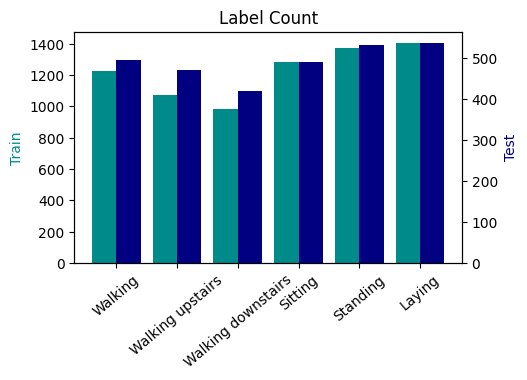
\includegraphics[width=0.95\columnwidth]{A_LabelCount.png}
            \caption{Número de amostras por classe.}
            \label{fig:numero_por_classe}
        \end{figure}

    \subsection{Dados Pré-processados}

        Os dados pré-processados estão normalizados no intervalo $[-1;1]$, à exceção de alguns dos atributos (figura \ref{fig:dados_preprocessados}). Desta forma, em um primeiro momento não existe necessidade de normalizar os dados.

        \begin{figure}[hbt!]
            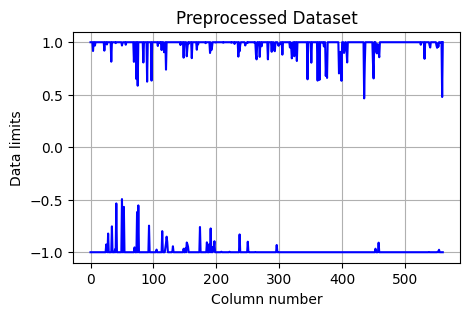
\includegraphics[width=0.95\columnwidth]{A_Dataset_Scale.png}
            \caption{Limites dos atributos do conjunto de treinamento dos dados pré-processados.}
            \label{fig:dados_preprocessados}
        \end{figure}

    \subsubsection{Regressão Logística}

        O classificador de regressão logística foi construído com a classe \href{https://scikit-learn.org/stable/modules/generated/sklearn.linear_model.LogisticRegressionCV.html}{\textbf{LogisticRegressionCV}} do \emph{Scikit-Learn}. Esta classe realiza a otimização do parâmetro de regularização junto com validação cruzada. Foram utilizadas as seguintes opções para o ajuste deste modelo:

        \begin{enumerate}
            \item Validação cruzada estratificada em 5 pastas.
            \item Normalização do tipo $l_2$ ($\frac{1}{2} ||w||_2^2$), com otimização do seu inverso ($c = \frac{1}{l_2}$)
            \item Função objetivo da otimização: acurácia balanceada.
            \item Estratégia: multinomial (entropia cruzada\footnote{Equivalente a utilizar \emph{Softmax}.}).
        \end{enumerate}

        O modelo ajustado tem $l_2 = 0.3594$. A acurácia balanceada na validação cruzada foi de $0.9932$, e com os dados de teste $0.9598$. Observa-se que o classificador tem um bom desempenho, e que o F1-score também seria uma boa escolha para avaliar a qualidade dos classificadores. (tabela \ref{tab:resultados_logistico_preprocessados}).

        Ao analisar por classe, fica claro que o desempenho não é uniforme. A classe \textbf{Sentado} tem um valor de \emph{recall} bem mais baixo que as demais, pois o classificador tem dificuldade em distinguir \textbf{Sentado} de \textbf{Em pé} (figura \ref{fig:cm_logistico_preprocessados}).

        \begin{table}[h]
            \centering
            \begin{tabular}{l c c}
                \toprule
                \textbf{Classe} & \textbf{\emph{Recall}}  & \textbf{\emph{F1 score}} \\
                \midrule
                Todas\tablefootnote{\emph{Recall} médio é a acurácia balanceada.}  & $0.9598$ & $0.9606$ \\
                \addlinespace
                Caminhar   & $0.9940$ & $0.9686$ \\
                Subir escadas   & $0.9427$ & $0.9569$ \\
                Descer escadas & $0.9690$ & $0.9795$ \\
                Sentado   & $0.8717$ & $0.9214$ \\
                Em pé  & $0.9812$ & $0.9372$ \\
                Deitado    & $1.0000$ & $1.0000$ \\
                \bottomrule
            \end{tabular}
            \caption{Resultados do classificador com regressão logística para os dados pré-processados.}
            \label{tab:resultados_logistico_preprocessados}
        \end{table}

        \begin{figure}[hbt!]
            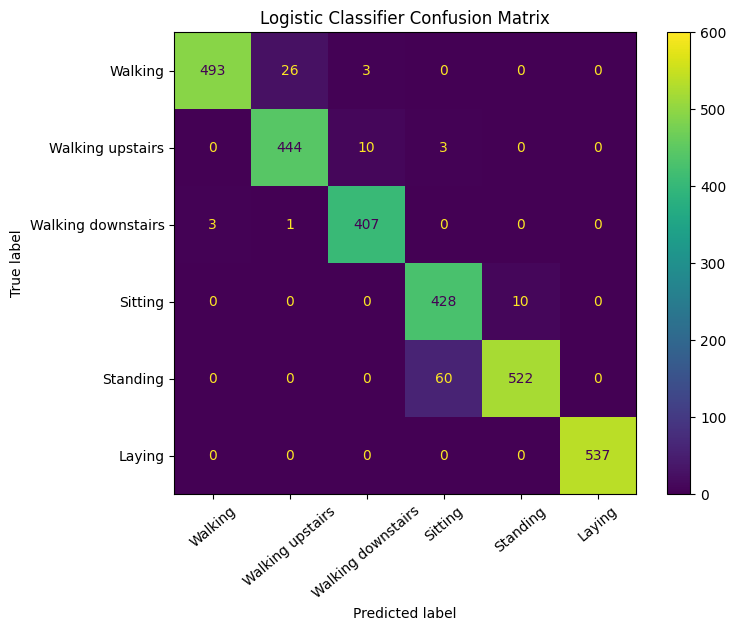
\includegraphics[width=0.95\columnwidth]{A_Logistic_CM.png}
            \caption{Matriz de confusão do classificador com regressão logística para os dados pré-processados.}
            \label{fig:cm_logistico_preprocessados}
        \end{figure}

    \subsubsection{k-Vizinhos mais Próximos}

        Na primeira tentativa de construção de um classificador com k-Vizinhos mais Próximos (\emph{kNN}) foram utilizadas as opções padrão da classe \href{https://scikit-learn.org/stable/modules/generated/sklearn.neighbors.KNeighborsClassifier.html}{KNeighborsClassifier} do \emph{Scikit-Learn}: distância euclidiana e pesos uniformes. Novamente foi utilizada a validação cruzada estratificada em 5 pastas.

        O valor ótimo de \textbf{k} ficou em 17 (figura \ref{fig:knn_melhor_k_preprocessados}). Este classificador com opções padrão (\emph{Vanilla}) ficou com acurácia balanceada na validação cruzada igual a $0.8999$, e com os dados de teste igual a $0.8999$\footnote{A coincidência de valores levantou suspeitas quanto ao código desenvolvido. O código foi verificado mais de uma vez, e nenhum erro foi encontrado. Os valores diferem na quinta casa decimal.}. Este classificador teve resultados inferiores ao do classificador com regressão logística (tabela \ref{tab:resultados_knn_vanilla_preprocessados}). Os resultados foram priores em todas as classes.

        \begin{figure}[hbt!]
            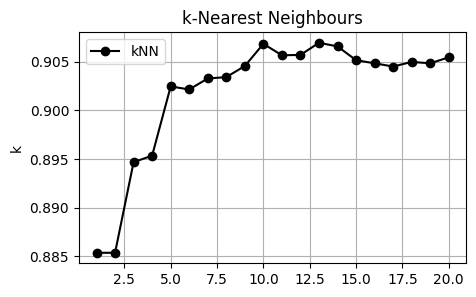
\includegraphics[width=0.95\columnwidth]{A_kNN_bestK.png}
            \caption{Otimização do parâmetro \textbf{k} do classificador com k-Vizinhos mais Próximos para os dados pré-processados.}
            \label{fig:knn_melhor_k_preprocessados}
        \end{figure}

        \begin{table}[h]
            \centering
            \begin{tabular}{l c c}
                \toprule
                \textbf{Classe} & \textbf{\emph{Recall}}  & \textbf{\emph{F1 score}} \\
                \midrule
                Todas & $0.8999$ & $0.9017$ \\
                \addlinespace
                Caminhar   & $0.9839$ & $0.9104$ \\
                Subir escadas   & $0.9108$ & $0.9022$ \\
                Descer escadas & $0.7667$ & $0.8530$ \\
                Sentado   & $0.7984$ & $0.8578$ \\
                Em pé  & $0.9436$ & $0.8885$ \\
                Deitado    & $0.9963$ & $0.9981$ \\
                \bottomrule
            \end{tabular}
            \caption{Resultados do classificador com k-Vizinhos mais Próximos para os dados pré-processados.}
            \label{tab:resultados_knn_vanilla_preprocessados}
        \end{table}

        \begin{figure}[hbt!]
            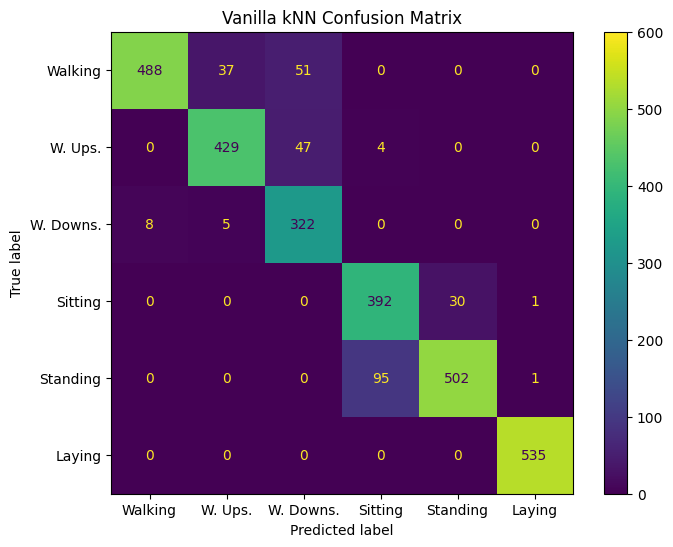
\includegraphics[width=0.95\columnwidth]{A_kNN_Vanilla_CM.png}
            \caption{Matriz de confusão do classificador com k-Vizinhos mais Próximos para os dados pré-processados.}
            \label{fig:cm_knn_vanilla_preprocessados}
        \end{figure}

        Dada a menor performance do classificador com k-Vizinhos mais Próximos, foram realizados alguns testes para tentar melhorar o seu resultado. A primeira tentativa foi uma busca em grade ao redor do melhor \textbf{k} encontrado, buscando os melhores hiperparâmetros para o classificador de k-Vizinhos mais Próximos. Foram testados diferentes valores de \textbf{p} para a métrica de Minkowski e o uso de pesos ponderados pelo inverso da distância (tabela \ref{tab:parâmetros_knn}). O classificador com os hiperparâmetros ótimos (\emph{kNN opt1}) mostrou um pequeno ganho na acurácia balanceada: $0.9045$ na validação cruzada e $0.9146$ nos dados de teste.

        \begin{table}[h]
            \centering
            \begin{tabular}{l c c}
                \toprule
                \textbf{Hiperparâmetro} & \textbf{Padrão (\emph{Vanilla})}  & \textbf{Otimizado} \\
                \midrule
                Distância    & Euclidiana & Manhattan \\
                Pesos    & Uniforme & Distância \\
                \bottomrule
            \end{tabular}
            \caption{Hiperparâmetros do classificador k-Vizinhos mais Próximos.}
            \label{tab:parâmetros_knn}
        \end{table}

        Como alguns dos dados de entrada não estava \emph{exatamente} escalados em [-1;1], a segunda tentativa foi aplicar uma escala [0;1] aos dados pré-processados. O resultado foi um pequeno incremento na acurácia balanceada: $0.9059$ na validação cruzada e $0.9153$ nos dados de teste.

        A última etapa na busca por um classificador com k-Vizinhos mais Próximos de melhores resultados foi avaliar os parâmetros de entrada. Foi feita uma otimização \emph{gulosa} dos parâmetros que são utilizados na construção do classificador de k-Vizinhos mais Próximos. A cada iteração são avaliados todos os parâmetros de entrada. A cada passo é retirado um dos parâmetros de entrada e o modelo é reconstruído. Se a acurácia balanceada aumentar, este parâmetro é retirado permamentemente. O algoritmo termina quando nenhum parâmetro é retirado em uma iteração.

        Para este estudo foi feita apenas uma iteração, ou seja, a retirada de cada atributo foi testada uma única vez. Este procedimento excluiu 65 dos 561 atributos, e levou a uma acurácia balanceada de $0.9218$ na validação cruzada e de $0.9192$ nos dados de teste.

        Uma possível etapa adicional seria a otimização do \emph{peso} de cada atributo. Este procedimento seria a otimização de 496 pesos. Devido ao custo computacional envolvido em uma otimização de tantos parâmetros, optou-se por considerar a avaliação concluída.

        Foi possível melhorar os resultados com relação a otimizar apenas o número de vizinhos, mas o incremento foi relativamente pequeno. Os resultados com os dados de teste geralmente seguiram os incrementos nos resultados com a validação cruzada. Em todas as tentativas os resultados ficaram abaixo daqueles do classificador com regressão logística.

    \subsection{Dados Brutos}

        Os dados brutos de aceleração e do giroscópio nas três direções levam a um conjunto de dados com 768 atributos. Os dados não estão normalizados (figura \ref{fig:dados_brutos}). Os dados pré-processados estavam \emph{aproximadamente} em $[-1;1]$ e foi pequeno, para o modelo de k-Vizinhos mais Próximos, o ganho de mudar a escala para $[0;1]$. Os dados brutos foram escalados para $[-1;1]$.

        \begin{figure}[hbt!]
            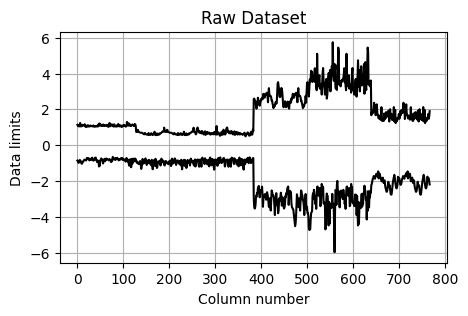
\includegraphics[width=0.95\columnwidth]{B_Dataset_Scale.png}
            \caption{Limites dos atributos do conjunto de treinamento dos dados brutos.}
            \label{fig:dados_brutos}
        \end{figure}



    \subsubsection{Regressão Logística}

    \subsubsection{k-Vizinhos mais Próximos}


\section{Conclusão}


\appendix

% \section{Lista de Variáveis}

    % \begin{description}
    %     \item[$X$:] xxxxxxxxxxx.
    % \end{description}


%% \section{}
%% \label{}

%% If you have bibdatabase file and want bibtex to generate the
%% bibitems, please use
%%

\bibliographystyle{elsarticle-num}
\bibliography{refs}

%% else use the following coding to input the bibitems directly in the
%% TeX file.

% \begin{thebibliography}{00}

%% \bibitem{label}
%% Text of bibliographic item

% \bibitem{}

% \end{thebibliography}


\end{document}
\endinput
